%----------------------------------------------------------------------
% Problem 2

\begingroup
\allowdisplaybreaks

\newpage
\section{Problem 2}

\textbf{Exercise 4 in Section 3.6}

\subsection{Solution}

\textbf{NOTE: } \textit{I do not have any experience in seismology, please forgive any mistakes in technicalities when I try to explain this exercise in my own words. It helps me understand what is going on so I can set up the problem correctly.}
\newline

The forward problem in this exercise allows mechanical waves to propagate through a $16 \times 16$ meter grid where each square in the grid have some slowness value $s_{x,y}$ in units of \unit{\second\per\meter}. Stations around the grid record time of arrivals of the mechanical waves as they pass through one or multiple grid squares. The time it takes to pass through a path of squares is formulated below.

\begin{align*}
	t &= \int_l s\left(\bv{x}\right) dl \\
	\\
	&\approx \sum_{blocks} s_{block} \Delta l
\end{align*}


\subsubsection{Part A - Row and Column Scans Only}

$16$ row scans and $16$ column scans are utilized in this part in the exercise as shown in figure \ref{fig: prob2 row column scan viz}. 

\begin{figure}[h] 
	\centering
	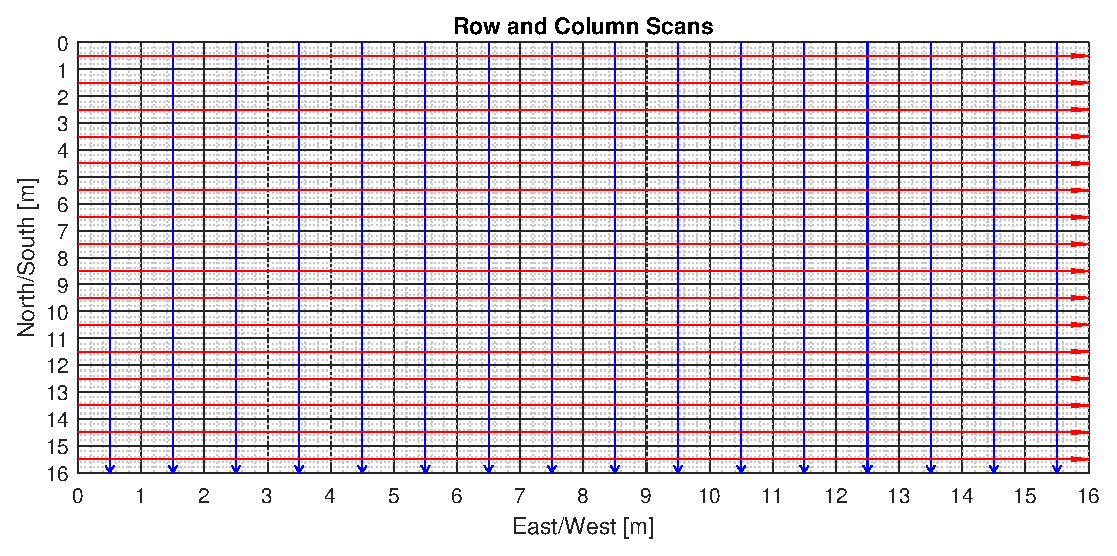
\includegraphics[width=0.85\textwidth]{./images/prob2_partA_scans_vizualization.eps}
	\caption{Row and Column Scan Visualization}
	\label{fig: prob2 row column scan viz}
\end{figure}
\FloatBarrier

This results in a total of $m = 32$ measurements. In an effort to estimate the slowness of each square in the grid, this results in a number of $n = 256$ model parameters. 

\begin{align*}
	\bv{d} \in \R^{32},\,\,\,\,\,\bv{m} \in \R^{256},\,\,\,\,\,G \in \R^{32 \times 256}
\end{align*}

The vector of measurement observations $\bv{d}$ is organized such that

\begin{align*}
	\bv{d} = \begin{bmatrix}
		t_{r,1} & t_{r,2} & \ldots & t_{r,16} & t_{c,1} & t_{c,2} & \ldots & t_{c,16}
	\end{bmatrix}^T
\end{align*}

where a $r$ subscript indicates a row can and a $c$ subscript indicates a column scan. The model parameters $\bv{m}$ are organized such that

\begin{align*}
	\bv{m} = \begin{bmatrix}
		s_{1,1} & s_{1,2} & \ldots & s_{1,16} & s_{2,1} & s_{2,2} & \ldots & s_{16,1} & \ldots & s_{16,16}
	\end{bmatrix}^T
\end{align*}

where the first subscript indicates the row, and the second subscript indicates the column. Each row of the model operator $G$ contain the distance traveled by the mechanical wave for each square in its path. Due to the large number of elements, a color map of the zeros and ones for this part of the problem as given instead in figure \ref{fig: prob2 model operator G}.

\begin{figure}[h] 
	\centering
	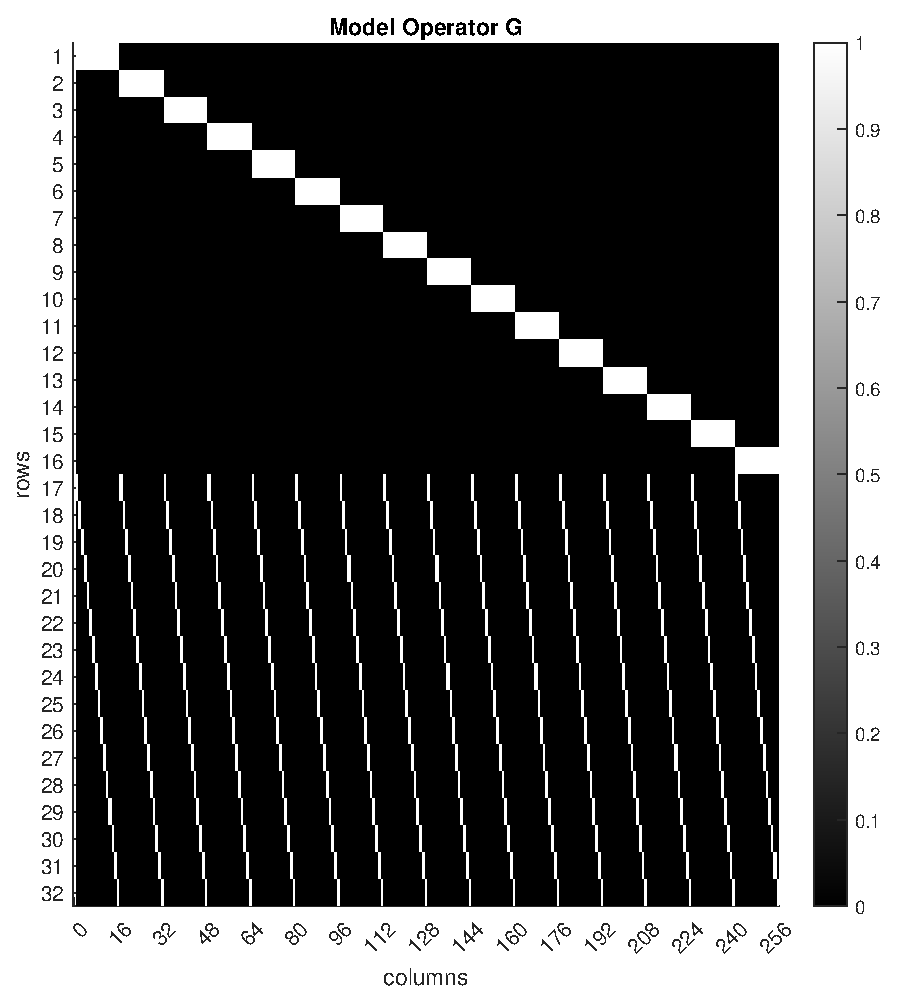
\includegraphics[width=0.85\textwidth]{./images/prob2_partA_model_operator_G.eps}
	\caption{Row and Column Scan Visualization}
	\label{fig: prob2 model operator G}
\end{figure}
\FloatBarrier

\textbf{Subpart A}

Per \MATLAB, the rank of G is $31$.

\textbf{Subpart B}


